% Use this template to write your solutions
\documentclass[12pt]{article}
\usepackage{fancyhdr}
\usepackage{amsmath}
\usepackage{amssymb}
\usepackage{relsize}
\usepackage{graphicx}
\usepackage[utf8]{inputenc}
\graphicspath{ {figures/} }

\usepackage{courier}

\usepackage[usenames,dvipsnames]{color} % Required for specifying custom colors and referring to colors by name
\usepackage[pdftex]{hyperref} % For hyperlinks in the PDF
\hypersetup{
  colorlinks=true,
  linkcolor=MyBlue, 
  citecolor=MyRed,
  urlcolor= MyBlue
}

\definecolor{MyRed}{rgb}{0.99, 0.0, 0.0} 
\definecolor{MyGreen}{rgb}{0.0,0.4,0.0} 
\definecolor{MyBlue}{rgb}{0.0, 0.0, 0.6}



% Set the margins
%
\setlength{\textheight}{8.5in}
\setlength{\headheight}{.2in}
\setlength{\headsep}{.25in}
\setlength{\topmargin}{0in}
\setlength{\textwidth}{6.5in}
\setlength{\oddsidemargin}{0in}
\setlength{\evensidemargin}{0in}



% Macros
\newcommand{\myN}{\hbox{N\hspace*{-.9em}I\hspace*{.4em}}}
\newcommand{\myZ}{\hbox{Z}^+}
\newcommand{\myR}{\hbox{R}}
\newcommand{\txt}[1]
{\textnormal{#1}}

\newcommand{\prob}[1]
{\textbf{P}\{{#1}\}}

\newcommand{\E}[1]
{\textbf{E}[{#1}]}

\newcommand{\mi}[1]
{\txt{min}_{#1}}

\newcommand{\ma}[1]
{\txt{max}_{#1}}

\newcommand{\myfunction}[3]
{${#1} : {#2} \rightarrow {#3}$ }

\newcommand{\myzrfunction}[1]
{\myfunction{#1}{{\myZ}}{{\myR}}}

% changing lists to (a), (b), (c) instead of 1. 2. 3. 
\renewcommand{\labelenumi}{(\alph{enumi})}

% Formating Macros

\newcommand{\myheader}[2]
{\vspace*{-0.5in}
\noindent
{#1} 

\noindent
{#2} 
\noindent
}  % end \myheader 

\newcommand{\courseheader}
{
\bf{COS 598C Spring 2015}
}

\newcommand{\authorheader}
{
Kiran Vodrahalli and Yanchen Wang
}

% Running head (goes at top of each page, beginning with page 2.
% Must precede by \pagestyle{myheadings}.
\newcommand{\myrunninghead}[2]
{\markright{{\bf{#1}: \txt{#2}}}}

\newcommand{\kiranhead}
{
 \lhead{\courseheader}
 \rhead{\authorheader}
}


\newcommand{\mytitle}[1]
{\begin{center}
{\large {\bf {#1}}}
\end{center}}

\newcommand{\probnum}[1]
{\large {\bf Problem {#1}}}

\newcommand{\mysection}[1]
{\noindent {\bf {#1}}}

%%%%%% Begin document with header and title %%%%%%%%%%%%%%%%%%%%%%%%%


\begin{document}
\pagestyle{fancy}

\kiranhead

[Primary Pedagogical Value: The main takeaway of this assignment is the idea that checking results from papers through your own implementation is a great skill to have. Acquiring the data and writing the code can be time-consuming, but if you research in the area, it can be worth it to check the facts stated in papers yourself. Secondarily, it is always important to compare more complicated methods suggested in papers to simpler, classical approaches, or at least have the knowledge that they do not work for a specific problem. This reason is why we include tasks involving $k$-means clustering and Canny edge detection on the problem set. The theme of this problem set can therefore be summarized as ``Neural Nets vs. Classical Methods".]

\vspace{0.5in}

\probnum{1}

The goal in this problem will be to explore methods of combining bounding box proposals to classify objects and form predictions about where they are located in a picture. We will be using the Overfeat paper as well as the SUN09 dataset. A set of images from the SUN09 dataset has been provided in your starter code. 

\begin{enumerate}

\item First, download a set of object proposals from \href{http://people.csail.mit.edu/myungjin/HContext.html}{$\txt{HContext.html}$}: You will need the \href{http://groups.csail.mit.edu/vision/Hcontext/data/detectorOutputsText.tar.gz}{detectorOutputsText.tar.gz} file. First you will need to gzip and untar the folders. These files are organized into two folders, \texttt{train} and \texttt{test}, each with subdirectories each specifying an object. Each of these object directories contains many .txt files named after the image to which the object belongs. Each line in the file contains bounding box locations and scores for that image in the format $[x_1 \txt{ } y_1 \txt{ } x_2 \txt{ } y_2 $\texttt{ score}$]$. Please apply the \texttt{exp} function to the scores so that all scores are positive. 

Your first task is to write a Python script transform this directory into a directory that instead contains a directory for each image in the image set provided, with a set of files for each image containing bounding box information. These files should be labeled $\{$\texttt{object name}$\}$.txt. Note: The \texttt{os} module is necessary for this task. Another useful module may be the \texttt{shutil} module. For drawing, you may want to use the \texttt{Image} and \texttt{ImageDraw} submodules from the \texttt{PIL} module.

Then, for each image, plot all bounding box proposals on top of the image for the following classes: \texttt{chair, books, wall, clock,} \texttt{door, drawer, shelves,} 
\texttt{television,} \texttt{window} (we restrict the set of object classes to plot so that it is reasonable to display a small number). Use a different color for each class you plot, and symbolize the confidence by varying the thickness of the lines the box is drawn with. (Include a legend specifying which color pertains to which category.) Use a different picture for each object class. 

[Justification for the problem: Sometimes in research and data analysis, datasets are not provided in a nice format and we have to reformat them. Learning how to use useful tools like Python for this sort of task is a useful skill for any researcher who works with data. The visualization portion of the task is important as well for conceptualizing the task individually.]

\item For each provided image, implement parts $(d)-(g)$ of the greedy merge algorithm for the proposed bounding boxes, as described on pages $10-11$ of the \href{http://arxiv.org/pdf/1312.6229v4.pdf}{Overfeat paper}. You will need to use the bounding box data from both the \texttt{train} and \texttt{test} folders. In the paper, they discuss the scale $s$: ignore this aspect of the algorithm, and assume that the bounding boxes of the same class for each image are all the proposals that exist. Be sure to explain and justify your implementation of \texttt{match$\_$score}, as only the idea of this algorithm is provided in the paper. Also be sure to assign a confidence score to the resulting merged bounding boxes based on the confidences of the individual bound scores (read pg. $11$ closely). Display the merged bounding box for each object class on top of the image as in part $(a)$.

[Justification for the problem: It is important to be able to read a paper and implement algorithms from a simple, sometimes incomplete description and evaluate it for yourself. This question is a simple exercise in implementing a simple algorithm where some information was left out, requiring the reader of the paper to think about and fill in the gaps. ]

\item The task will be to perform an experiment to see how well a common clustering algorithm can distinguish object classes based on bounding boxes. You will apply $k$-means clustering on each object class of bounding boxes for an image as a replacement to the method defined in the Overfeat paper. Think carefully about how to define a vector for each bounding box: recall that $k$-means minimizes distortion, or the sum of the squared Euclidean distances between each bounding box vector and the centroid it is closest to. A na{\"i}ve approach would simply specify each bounding box as a $4$-tuple $(x_1, y_1, x_2, y_2)$. What distance are we trying to minimize between bounding boxes? You might use the approach from part $(b)$ as inspiration. Feel free to choose the number of dimensions in your representation. Give justification for your bounding box representation. You may find the Python module \href{http://docs.scipy.org/doc/scipy/reference/cluster.vq.html}{\texttt{scipy.cluster.vq}} useful (do not implement your own version of $k$-means). Don't forget to draw the resulting clustered bounding boxes on the images!

[Justification for the problem: Researchers should constantly think about valid approaches to solve problems in papers they read apart from the solutions prevented. This question has the dual benefit of introducing $k$-means and causing the student to think about the representation problem. Representing something as simple as a bounding box can be done in many ways. It also requires the student to think about the optimization problem at hand, in terms of norms and objectives. The goal here is not for the student to have to implement $k$-means. Good answers will come up with a sensible vector representation, with coordinates potentially involving the Jaccard similarity (an area-based metric), distance between bounding box centroids, possibly even the confidence scores.]


\end{enumerate}

\probnum{2}

The task will focus on the segmentation task from \href{http://people.idsia.ch/~juergen/nips2012.pdf}{Ciresan, Giusti, Gambardella, and Schmidhuber}. We use the ISBI $2012$ Challenge Data dataset.

\begin{enumerate}

\item First, download the dataset. The ISBI $2012$ Challenge data are downloadable from \href{http://brainiac2.mit.edu/isbi_challenge/home}{$\txt{http://brainiac2.mit.edu/isbi\_challenge/home}$}. After registering an account, you can download the data from the ``Downloads" section. The images are all in \texttt{.tif} format, of dimension $512 \times 512$ pixels. Three sample images from the dataset are presented in \autoref{fig:trainlabeltest}. 
\begin{figure}
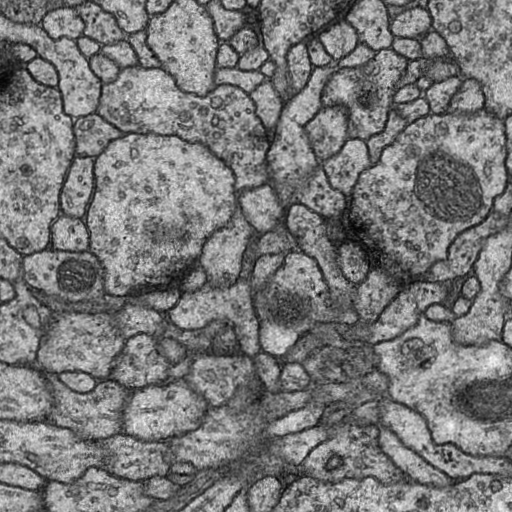
\includegraphics[scale=0.2]{trainvolume}
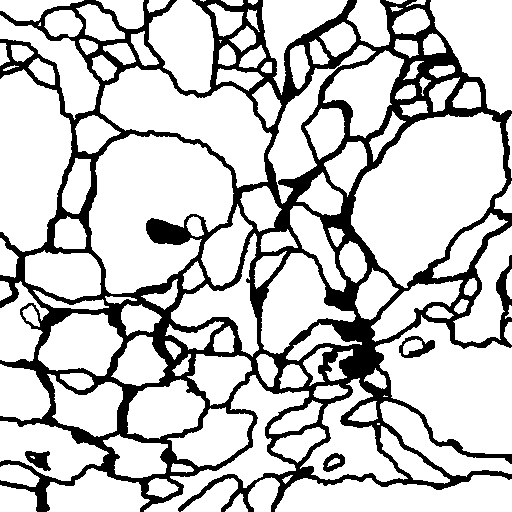
\includegraphics[scale=0.2]{trainlabels}
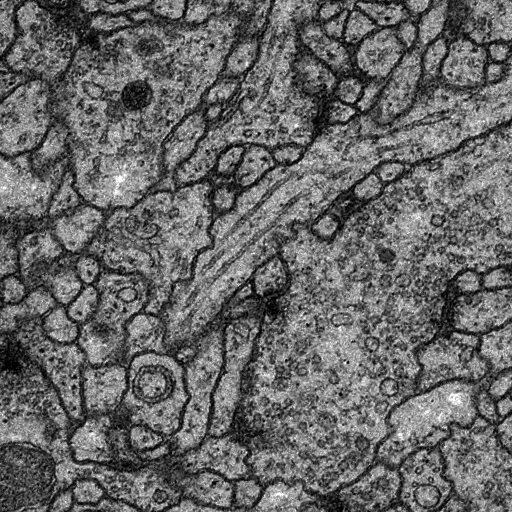
\includegraphics[scale=0.2]{testvolume}
\centering
\caption{A training image, the associated label, and a test image.}
\label{fig:trainlabeltest}
\end{figure}

In fact, we had difficulty downloading the data set because the website indicated we were robots, not humans. Perhaps future TAs for this course can simply directly give the students this data set because some students may experience the same bug.

\item The paper defines several convolutional neural networks to learn segmentations of neurons. This part of the question requires you to implement the N$4$ network from pg. $6$ in code. Specifically, please use the \href{http://deeplearning.net/software/theano/}{\texttt{theano}} Python module. You may find it helpful to use \href{http://lasagne.readthedocs.org/en/latest/}{\texttt{lasagne}} module, which is built on top of \texttt{theano}. 

[Justification for the problem: As in Question $1$, researchers should have the skill to implement software specifications given in papers. Since the course is focused on neural nets, it follows that any student completing the course should be able to implement in code a neural net architecture they come across in a paper to evaluate for themselves. It is also important to be able to replicate the test metrics used in the problem.]

\item Evaluate the pixel error and the rand error defined in the paper for the dataset. 

[Justification for the problem: It is important to be able to implement metrics given in the paper, and to evaluate them on the data presented in the paper to check figures.]

\end{enumerate}


\probnum{3}

This problem is in some ways a continuation of Problem $2$. The task is to first implement and then apply the Canny edge detector to the ISBI $2012$ dataset, and to compare its performance to the neural net implemented in part $2(a)$. We now walk through the implementation of a Canny edge dector in Python.

\begin{enumerate}

\item Implement Gaussian filter. 

\item Implement blahblah. 

\item Compare results to the neural net from Problem $2(a)$ using the metrics in Problem $2(b)$. 

\end{enumerate}

\vspace{0.1in}

\large\textbf{Contributions}

Kiran contributed the code for Problem $1$ and wrote up the document, and also implemented the Canny edge-detection in Problem $3$. 
Yanchen implemented the code for Problem $2$. We both discussed ideas for the assignments together and agreed on the problems together.


\end{document}
